% 编译：./build.sh；字体使用本机宋体，不随报告分发商业字体。
\documentclass[UTF8,a4paper,zihao=5,fontset=none,twoside]{ctexart}
\usepackage{fontspec}
\IfFontExistsTF{SimSun}{\setCJKmainfont[AutoFakeBold=2.5]{SimSun}}{\setCJKmainfont[BoldFont={Songti SC Bold}]{Songti SC}}
\setmainfont{Times New Roman}
\setCJKmonofont{Songti SC}
\usepackage[a4paper,top=2.5cm,bottom=2.5cm,left=3cm,right=3cm,headheight=14pt,headsep=\dimexpr1cm-14pt\relax,footskip=1cm,bindingoffset=0cm]{geometry}
\usepackage{setspace,graphicx,booktabs,tabularx,array,caption,float,fancyhdr,tikz,enumitem,hyperref}
\usetikzlibrary{arrows.meta,positioning,calc}
\newcolumntype{L}[1]{>{\raggedright\arraybackslash}p{#1}}
\renewcommand{\tabularxcolumn}[1]{>{\raggedright\arraybackslash}p{#1}}
\singlespacing
\setlength{\parindent}{2em}
\setlength{\parskip}{3pt}
\ctexset{section={format=\zihao{3}\bfseries,number=\chinese{section},aftername=、,beforeskip=12pt,afterskip=10pt},subsection={format=\zihao{4}\bfseries,beforeskip=9pt,afterskip=5pt},subsubsection={format=\zihao{-4}\bfseries},paragraph={format=\zihao{5}\bfseries}}
\captionsetup{font={normalsize},labelfont=bf,labelsep=quad,skip=6pt}
\setlist{nosep,leftmargin=2em}
\definecolor{ink}{HTML}{183449}
\definecolor{blue}{HTML}{287DB4}
\definecolor{pale}{HTML}{EFF5F8}
\pagestyle{fancy}\fancyhf{}
\fancyhead[C]{\zihao{5}MeetAgent 会合助手\quad 作品说明文档}
\fancyfoot[LE,RO]{\zihao{5}\thepage}
\renewcommand{\headrulewidth}{0pt}
\hypersetup{hidelinks,pdftitle={作品说明文档：MeetAgent 会合助手},pdfauthor={李祥熙}}
\newcommand{\shot}[3]{\begin{minipage}[t]{0.46\textwidth}\centering\includegraphics[height=11.2cm,width=\linewidth,keepaspectratio]{assets/#1}\par\vspace{5pt}\textbf{#2}\par #3\end{minipage}}
\begin{document}
\begin{center}
{\zihao{2}\bfseries 作品说明文档}\par\vspace{7pt}
{\zihao{2}\bfseries MeetAgent · 会合助手}\par\vspace{9pt}
{\zihao{3}\bfseries 李祥熙}\par\vspace{6pt}
队伍：为了看Miku演唱会特前来拿奖金\par
HarmonyOS 智能会合规划应用\par
2026 年 9 月
\end{center}
\section{创意描述}
综合司机路线、乘客可用出行方式与时间偏好，比较原地等待和移动会合方案，通过 AI 理解需求并解释结果，帮助双方确定会合地点。
\section{设计稿与交互流程}
\subsection{产品定位}
会合助手是一款面向司机与乘客接送场景的鸿蒙应用。用户在行程开始前输入双方位置和乘客出行偏好，应用比较不同会合点及出行方式，提供双方预计用时、路线和会合地点。确认后，用户可以分享方案并打开地图导航。
\subsection{操作流程}
应用设有地图、助手、行程和设置四个入口。地图用于选点与路线展示，助手用于自然语言输入，行程页保存已确认方案。普通规划和智能助手均使用相同的路线与方案比较能力。
\begin{figure}[H]\centering
\begin{tikzpicture}[font=\zihao{5},box/.style={draw=blue,fill=pale,rounded corners=3pt,text width=3.55cm,minimum height=1.4cm,align=center},arr/.style={-{Latex},thick,ink}]
\node[box](a){输入双方位置\\搜索 / 地图选点};
\node[box,right=0.55cm of a](b){设置乘客偏好\\方式 / 步行上限};
\node[box,right=0.55cm of b](c){生成会合方案\\路线与用时比较};
\node[box,below=0.65cm of c](d){查看方案详情\\地图 / 分段行程};
\node[box,left=0.55cm of d](e){确认并锁定方案\\保存会合地点};
\node[box,left=0.55cm of e](f){执行会合方案\\复制分享 / 打开地图};
\draw[arr](a)--(b);\draw[arr](b)--(c);\draw[arr](c)--(d);\draw[arr](d)--(e);\draw[arr](e)--(f);
\end{tikzpicture}
\caption{会合规划的主要操作流程}
\end{figure}
\subsection{界面组织}
位置输入与路线展示以地图为中心；步行、骑行、公共交通和原地等待以方案卡片呈现，便于比较。选择公共交通方案后，页面展示乘客分段行程。确认方案后，行程页集中显示会合点、双方路线及用时。
\clearpage
\section{介绍文档}
\subsection{需求背景}
在车站接人、校园接送等场景中，固定上车点可能增加司机绕行与等候时间。如果乘客能够步行、骑行或乘公共交通移动一段距离，双方可能在其他地点更早会合。会合助手将双方的时间与乘客移动负担纳入同一次规划。
\subsection{位置输入与出行偏好}
用户通过搜索或地图选点设置双方位置，再选择乘客可用方式、步行上限，以及综合最优或地铁优先策略。用户也可向智能助手输入“我可以骑车”“尽量少走路”等要求，由助手理解偏好并调用规划功能。
\begin{figure}[H]\centering
\shot{preferences.png}{规划设置}{出行方式、计算策略与步行上限。}\hfill
\shot{chat.png}{智能助手入口}{通过自然语言补充出行要求。}
\caption{结构化偏好设置与自然语言输入入口}
\end{figure}
\clearpage
\noindent\begin{minipage}[t]{0.48\linewidth}\vspace{0pt}
\subsection{会合方案比较}
\begin{minipage}[t][4.8cm][t]{\linewidth}
结果页保留原地等待方案，并列出可行的移动会合方式。每个方案显示会合位置、预计会合用时和司机节省时间，地图展示双方路线。

图~\ref{fig:comparison} 的西安示例中，原地等待预计为 80 分钟；推荐方案的司机用时为 35 分钟，乘客为 42 分钟，预计会合用时为 42 分钟，比原地等待减少 38 分钟。
\end{minipage}
\par\centering
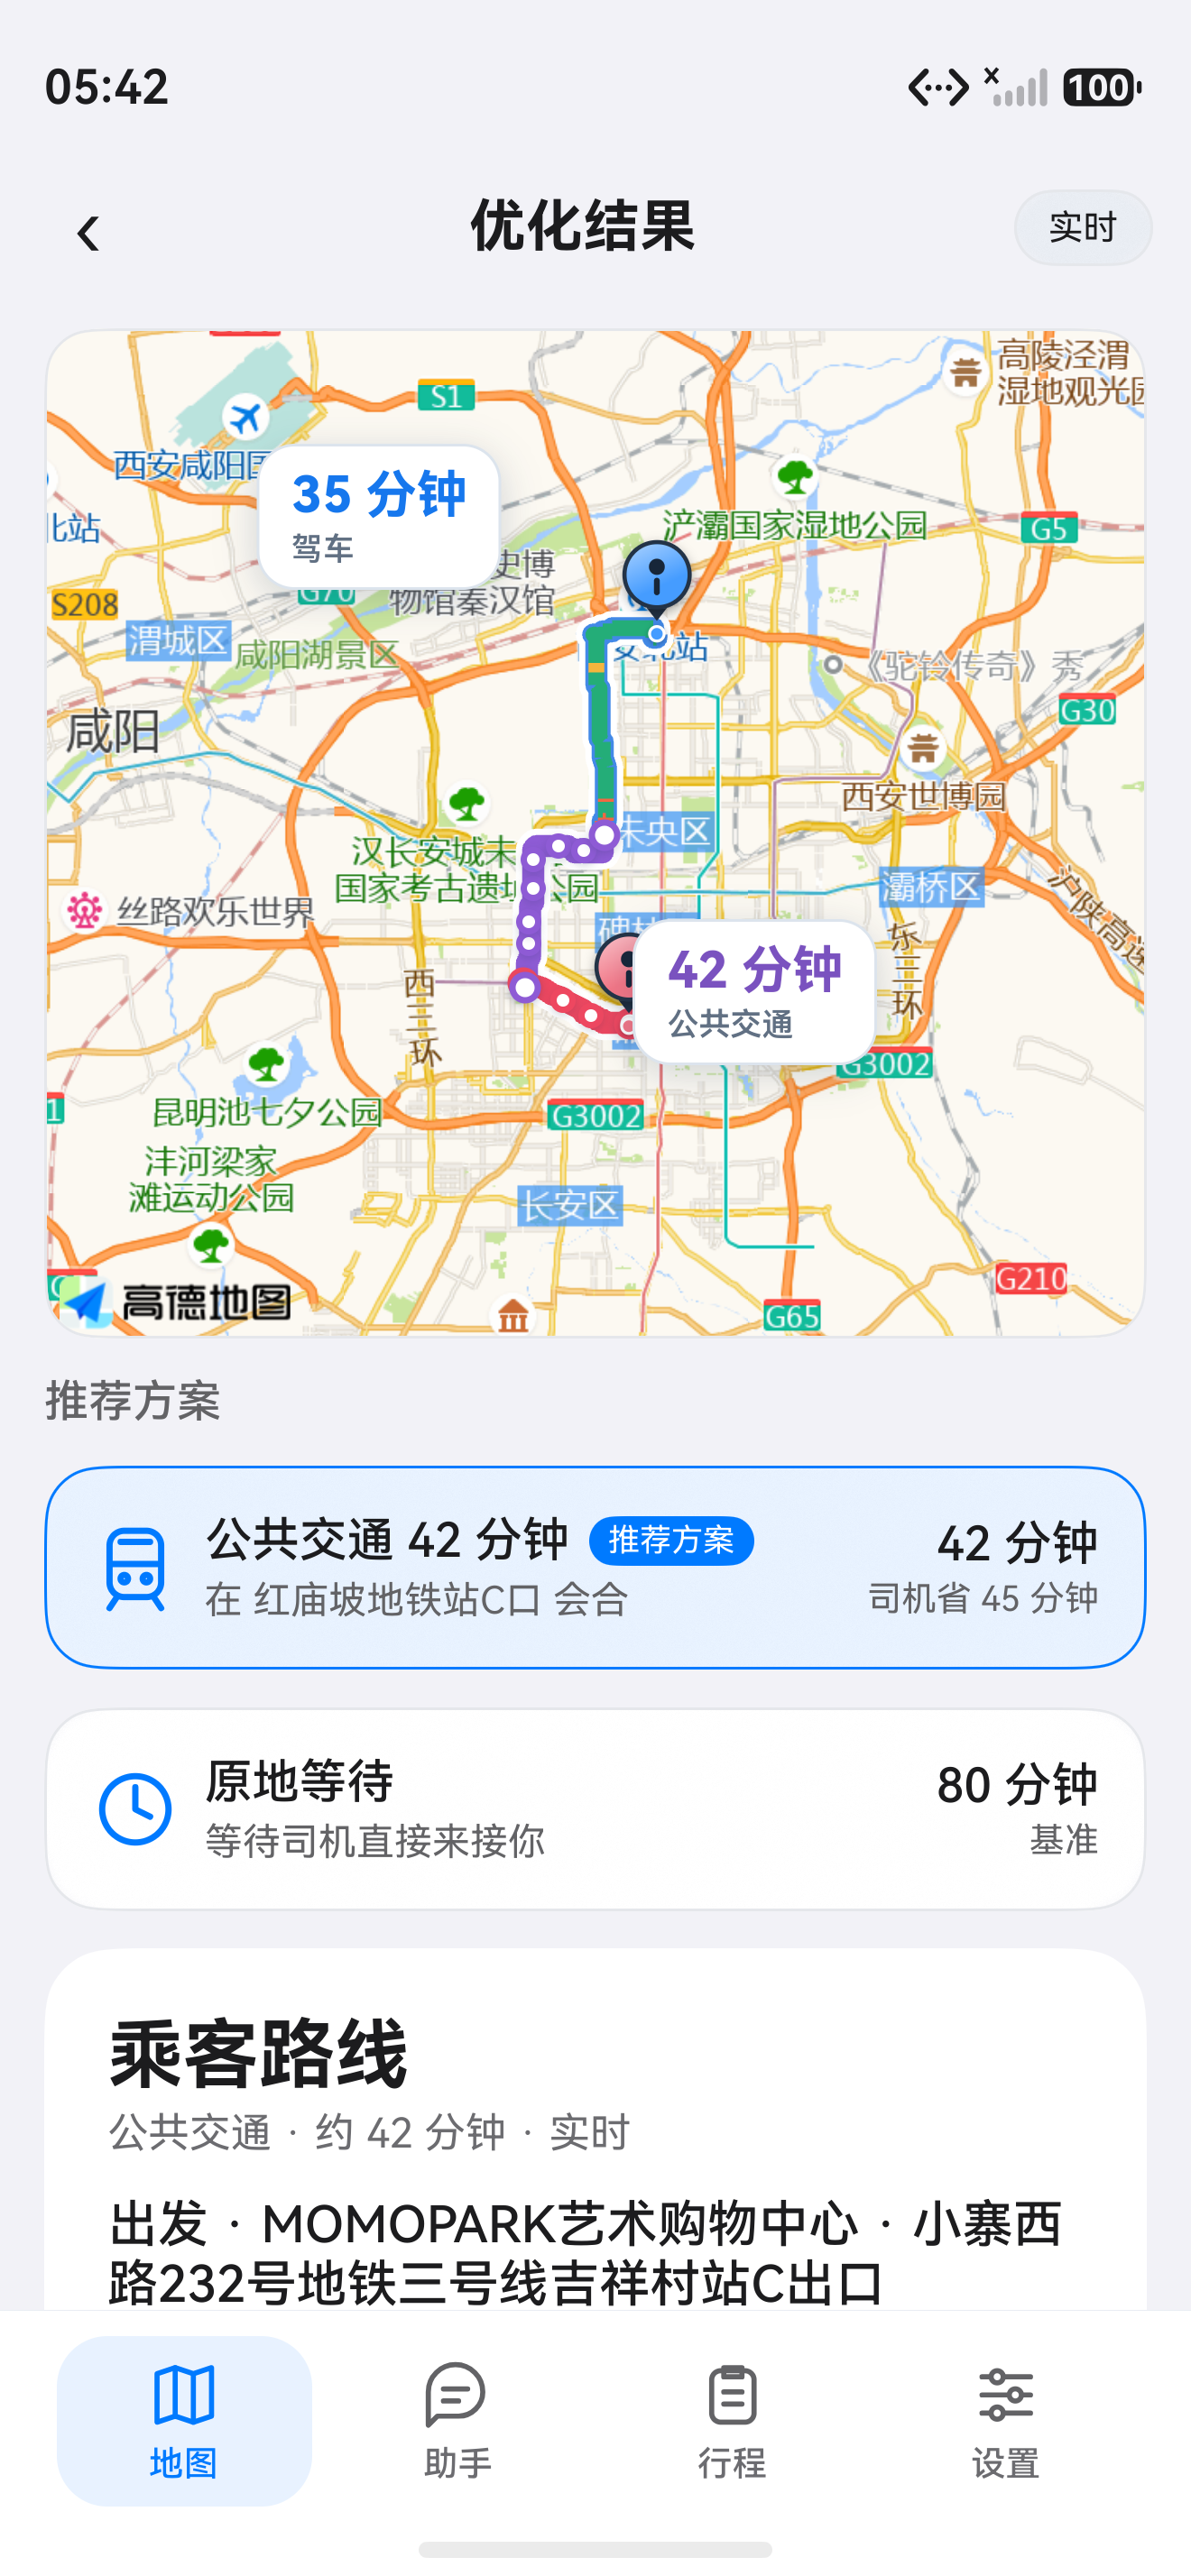
\includegraphics[height=12.8cm,width=\linewidth,keepaspectratio]{assets/plan.png}
\captionof{figure}{会合方案与双方路线比较}\label{fig:comparison}
\end{minipage}\hfill
\begin{minipage}[t]{0.48\linewidth}\vspace{0pt}
\subsection{公共交通路线详情}
\begin{minipage}[t][4.8cm][t]{\linewidth}
选择公共交通选项卡后，可查看乘客的具体路线。地图用不同颜色区分交通线路，页面下方按顺序列出地铁、步行与换乘步骤。

图~\ref{fig:transit} 展示了同一方案的分段行程，包括地铁 3 号线与 8 号线、上下车站、步行距离、预计用时和进出站口，便于乘客判断换乘与步行安排。
\end{minipage}
\par\centering
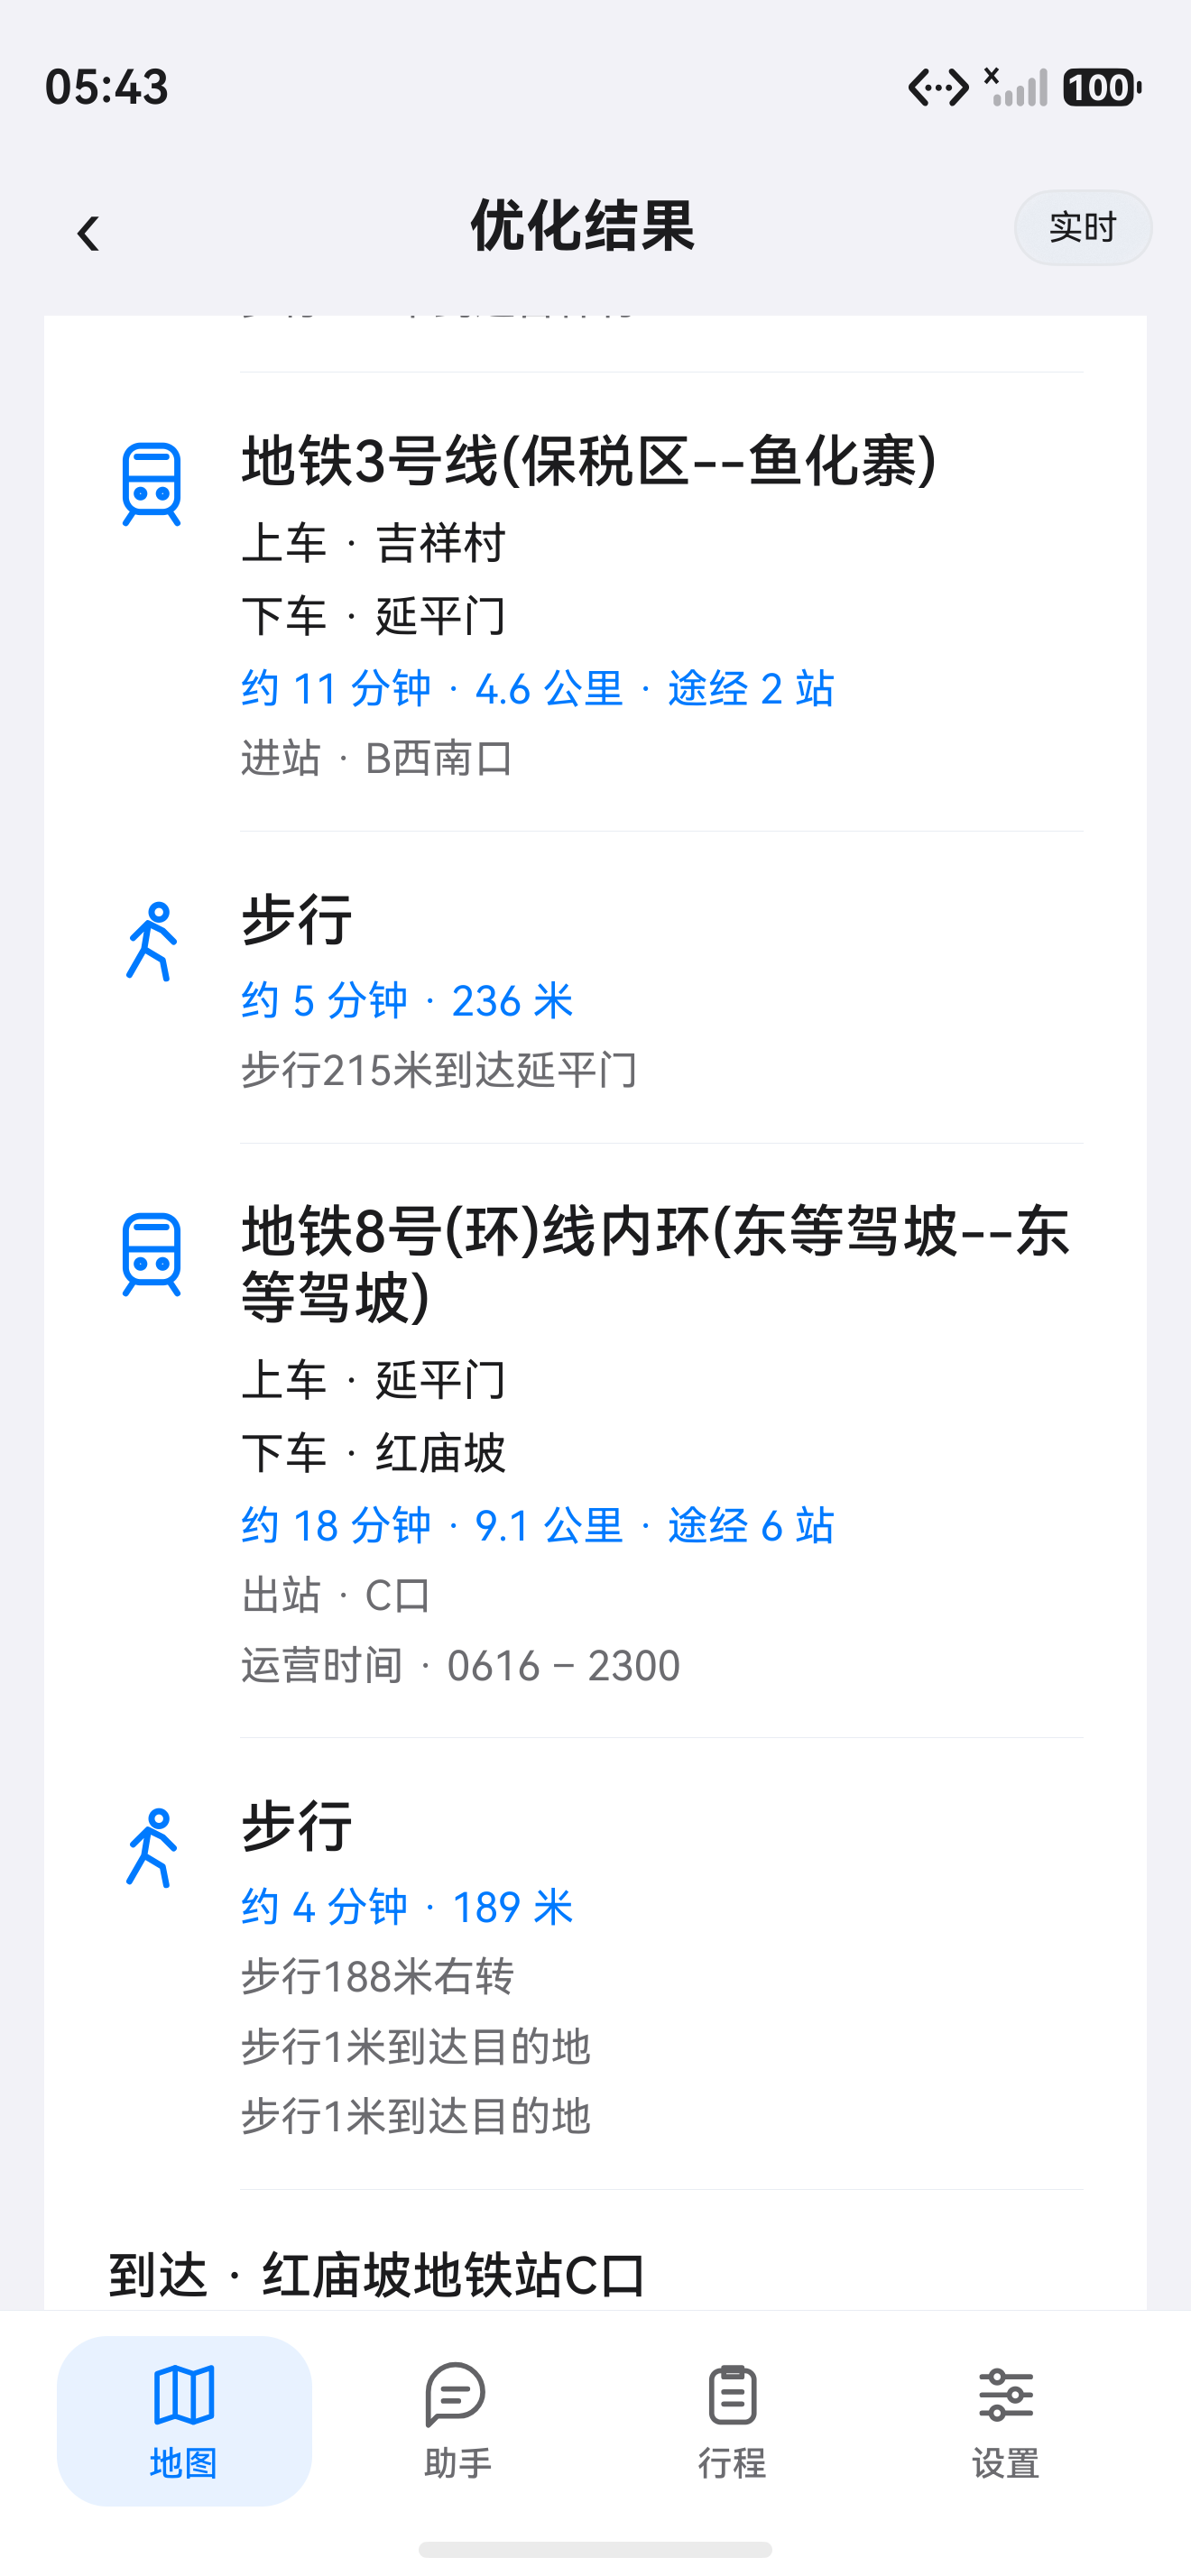
\includegraphics[height=12.8cm,width=\linewidth,keepaspectratio]{assets/passenger-route.png}
\captionof{figure}{公共交通方案的乘客分段行程}\label{fig:transit}
\end{minipage}
\par\vspace{12pt}
图~\ref{fig:comparison}、图~\ref{fig:transit} 为同一次模拟器运行的应用截图，数值为该次路线规划的预计结果。
\clearpage
\subsection{方案确认、分享与导航}
用户确认后，会合地点与路线保存在行程页，不会自动改变；调整地点时需主动重新规划。行程信息可复制分享给对方，并衔接地图导航。一部手机即可完成规划，对方通过分享内容了解会合安排。
\begin{figure}[H]\centering
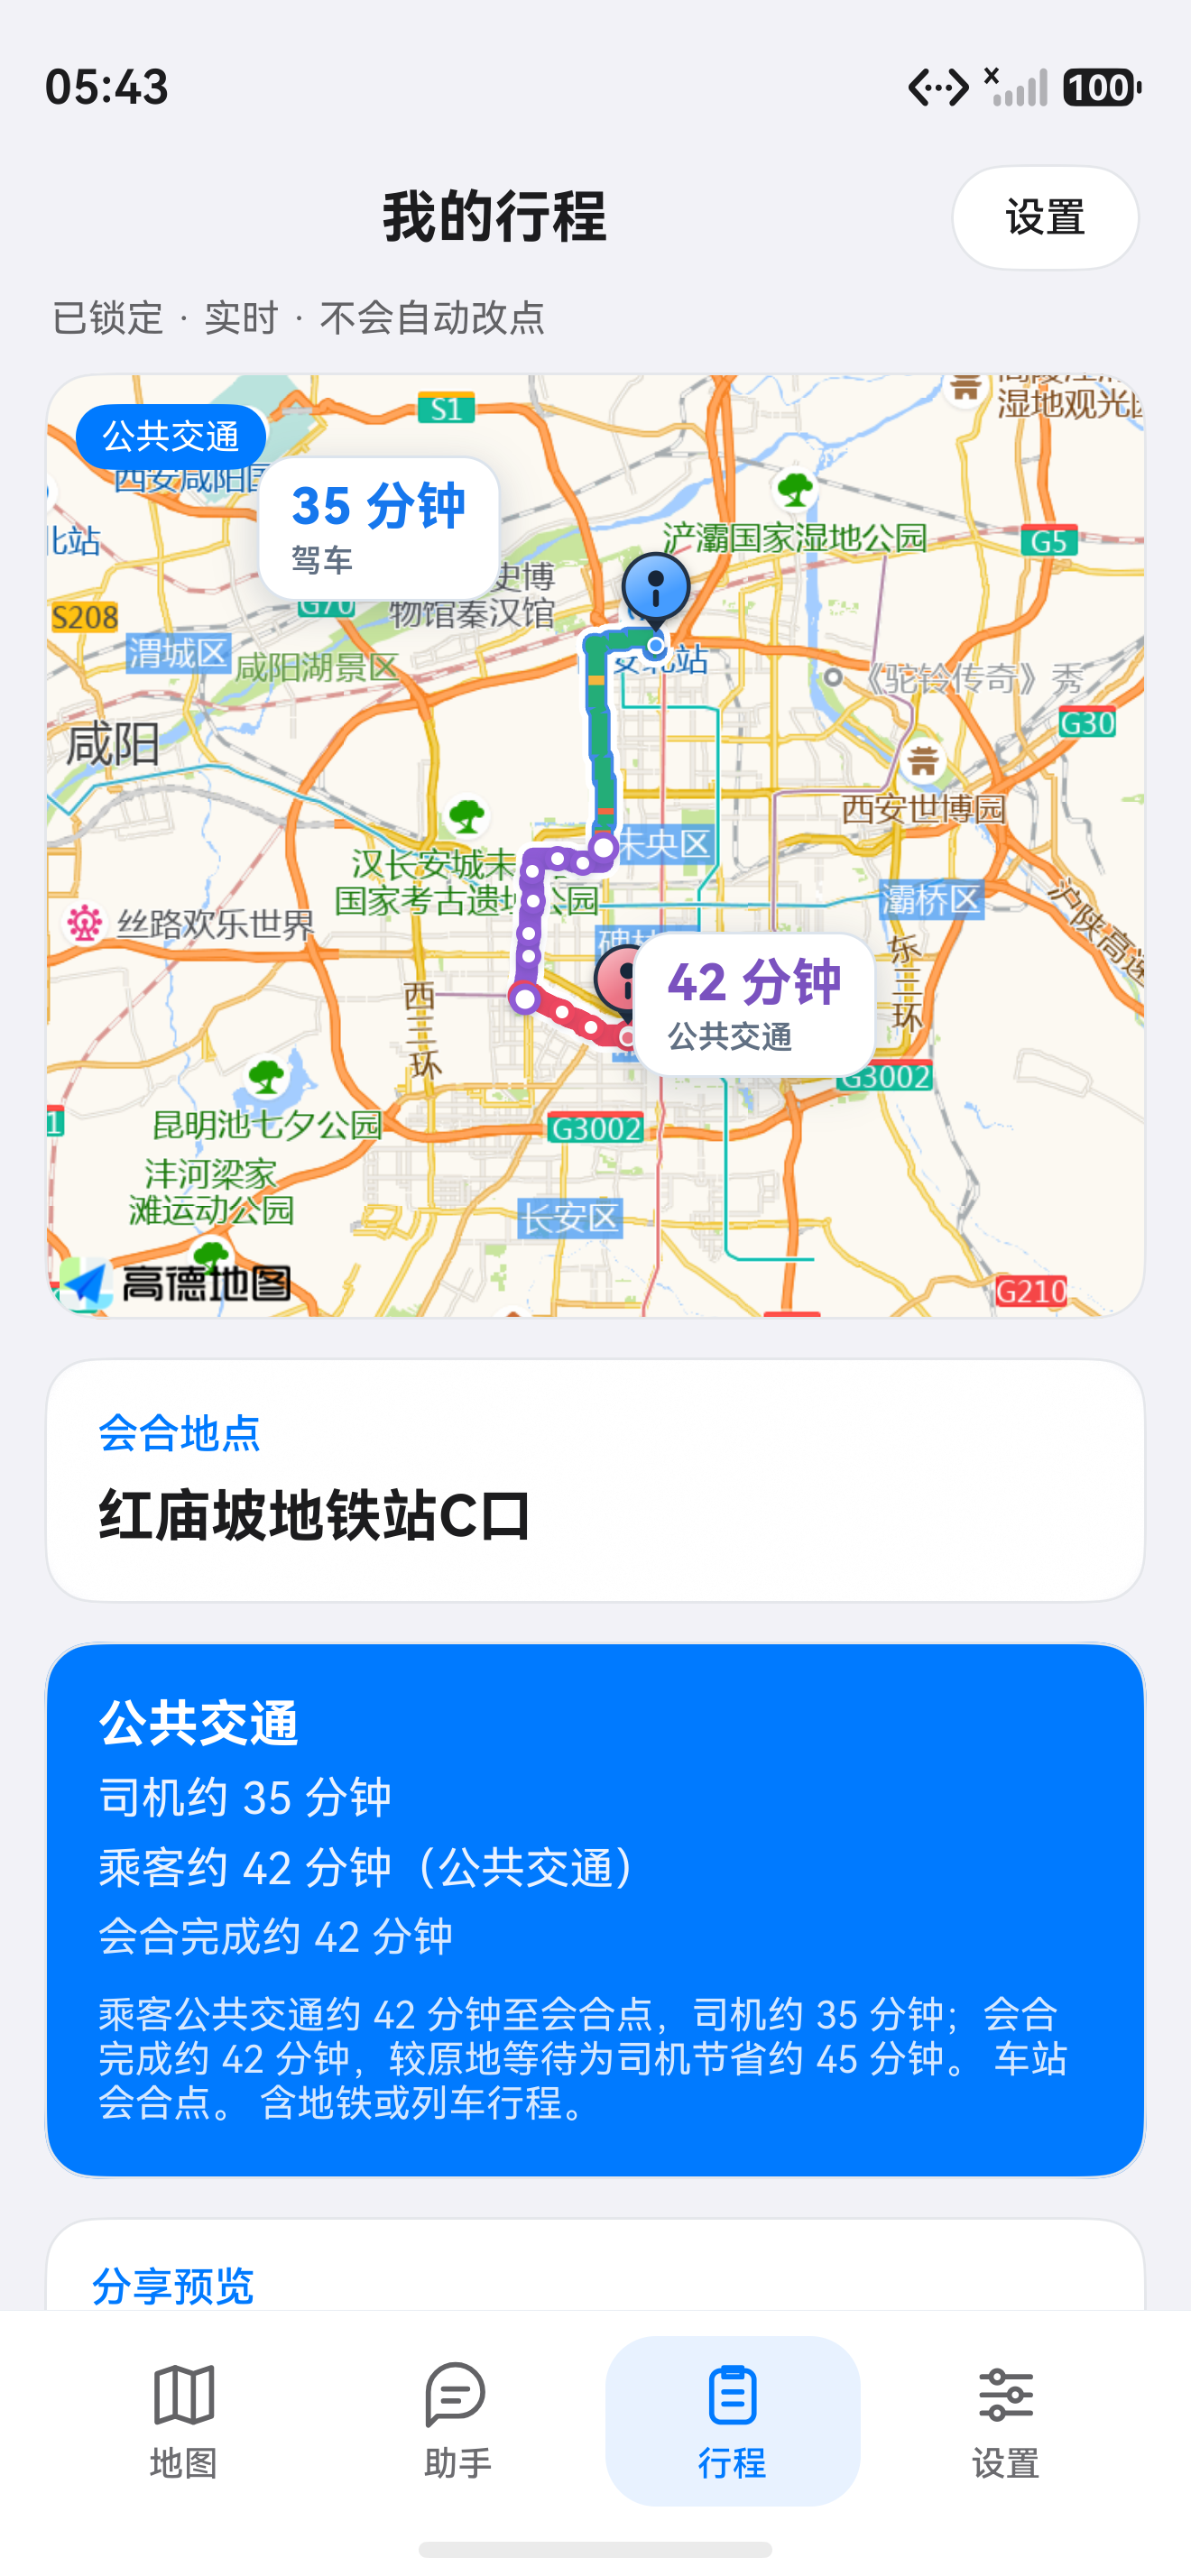
\includegraphics[height=12.5cm]{assets/locked.png}
\caption{确认后的行程页：会合地点、双方用时及路线}
\end{figure}
\subsection{功能实现}
应用采用 HarmonyOS 原生界面。地图服务提供路线和预计用时，本地规划引擎比较候选地点、双方到达时间及乘客移动负担；AI 负责理解偏好、调用工具和解释方案。没有足够改善时，应用推荐原地等待。普通规划可独立于 AI 服务使用。
\clearpage
\subsection{应用场景与发展前景}
会合助手适用于一方驾车、另一方具有短途移动条件的接送需求。其价值主要体现在：比较不同会合位置，减少单独查路线和协商地点的操作，并为乘客提供明确的到达步骤。
\begin{table}[H]\centering\caption{主要应用场景与对应需求}
\renewcommand{\arraystretch}{1.4}
\begin{tabularx}{\linewidth}{L{2.6cm}X}\toprule
\textbf{应用场景} & \textbf{对应需求}\\\midrule
亲友接送 & 结合司机路线和乘客出行意愿，提前确定双方可接受的会合地点。\\
校园与园区 & 比较不同出入口及周边位置，衔接司机驾车与乘客步行、骑行路线。\\
交通枢纽接送 & 利用车站周边公共交通，比较站外或沿途会合与直接到站接人的时间。\\
活动散场接送 & 在接送前比较周边候选位置，明确双方路线，减少临时寻找对方的沟通。\\\bottomrule
\end{tabularx}
\end{table}

后续可进行多机同步功能的开发，实时显示双方当前位置。或根据当前路况的变化选择推荐更优的会合点，以及加强校园接送场景的优化，精确到出入口等等。
\end{document}
